\chapter{Software development tools and concepts}
\label{progB}
The main deliverables of this project are two software artifacts.
\begin{enumerate} 
\item A Matlab application that visualises the generation of patterns obtained from the interconnections of cells.
\item An environment for testing process schedulers, including the implementation of a diffusion-inspired scheduler.
\end{enumerate}
Various programming and script languages were used. The first application is written in Matlab. The second application includes two parts: a process management framework written in Java on the Eclipse IDE and a set of bash scripts that use gnuplot \cite{gnuplot} to generate bar graphs for analysing and testing the various scheduler implementations.
Basic knowledge of the concepts, the languages and the algorithms used are provided throughout this chapter.  
	
\section{Matlab}
    
Matlab is a programming environment developed by MathWorks \cite{MATLAB_2010}. It is ideal for working with vectors and matrices since it has build in matrix operations. It provides basic and advanced mathematical procedures and functions, such as sin, cos, Fourrier transformations and ordinary differential equation solvers. Its capability of producing all kinds of graphs and supplying a plethora of image processing functions makes it the ideal tool for studying the phenomenon of morphogenesis.

The approach was to study and test models by solving differential equations and producing representational graphs and at the end, generating movies with image time frames to show how cells get organised and what shapes they produce. An example of such image frame is shown in Figure \ref{pattern}.
\begin{figure}[h!]
    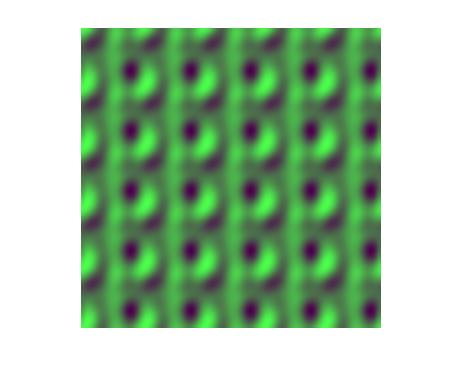
\includegraphics[scale=0.5]{pattern.png}
    \centering
    \caption{An image representation of the structure produced by a system of cells.} 
    \label{pattern}
\end{figure}   
    
The functions in Matlab are written according to the format below:
    \begin{lstlisting}[language=matlab]
        function <output> = name(<arguments>)
            body
        end
    \end{lstlisting}
    
    Note that the output can be a vector, a 2-dimensional array or an abstract structure, meaning that the type of the output value will be given during the execution of the program.  
	\subsection{Modelling morphogenesis}	
    
As explained in Chapter \ref{morphogenesis}, there are several dynamical models of the reaction-diffusion process in morphogenesis. The reaction model has the form $ \dot{x}=F(x) $ and the diffusion model is according to conduction of heat as explained in paragraph \ref{diffusion} with cell interconnections of ring or torus-shaped structures. The Matlab program that was generated to solve such a model has two main parts.
    
The first part is the main function, where the initial conditions are given. Those conditions are the number of cells, the initial concentrations of each chemical compound and the diffusion coefficients. The main function constructs the data structures - which are vectors - and calls the appropriate ODE solver with arguments a function, a column vector (as the initial conditions) and a time span. Other arguments that are used by the ODE algorithm are explained in the next paragraph. Any function can have inside the definition and implementation of another function which is called a nested function.
    
The main purpose of the nested function is to make sure that the implementation of the mathematical model is evaluated correctly. The equations of such a model should be implemented in the nested function in a way that the vector operations are evaluated correctly. From a software development point of view, using a nested function instead of an external one is better, since the defined constants are easily shared from the main to its nested function. An example of a template code for solving ordinary differential equations is shown in Figure \ref{templateCode}.
\begin{figure}[h!]
\begin{center}
    \begin{lstlisting}[language=matlab]
    function out = f()
        %body, initialise constants
        %call an ODE solver, such as ode45, ode23 etc...
        %example:
        [t, x] = ode45(@odefun, [0 100]); 
        %that will solve equations in a time span 0-100 seconds        
        
        plot x in respect to t as x(t(i))=x(i)
            
        function odefun = integration(tspan, init)
            body evaluate equations 
            ode = equation results (column vector)
        end
    end 
    \end{lstlisting}
\caption{Template of Matlab code for solving ODE's.}
\label{templateCode}
\end{center}
\end{figure}
	\subsection{Integrating ordinary differential equations}
    Matlab provides a variety of ODE solver implementations each of them having different properties. Note that there are some constraints in evaluating a model that describes fluid concentrations. The main constraint is that the concentrations must never get a negative value otherwise the model will have no physical meaning.

The ODE-solver used in this project is the \texttt{ode45}. According to the Matlab documentation \texttt{ode45} is for solving non-stiff differential equations of medium order and it is the most common used among the provided ode solvers \cite{MATLAB_2010}.
    
Apart from the ODE arguments shown on line 5 in Figure \ref{templateCode},
    the solver can also be given a structure of options as an extra argument. Options are used to override any default behaviour and explicitly define the constraints that the solver must take into account. The options are declared with the use of the \texttt{odeset} function.
    
The \texttt{odeset} function takes an arbitrary length of arguments. First, a string value is given which represents the key of the parameter that is intended to be overridden following by a real numerical value. For example, any reaction-diffusion model requires that no cell has a negative concentration of any of its morphogens. Thus, the options are constructed with the code below:
    $$ options = odeset('NonNegative',(1:N)); $$
    Where N is the size of the solution vector (cells$\times$morphogens). Note that all matlab ode solvers accept a column vector as the initial conditions and thus extra care should be taken for converting a 2-dimensional array to a column vector and the opposite correctly.
	 
	\subsection{Plotting the results}
    Matlab provides easy to use methods that make plotting graphs convenient. The interest lies on observing graphically the equilibrium points of the system, how the system oscillates and for how long. Thus, plotting the results helps in both the analysis of the system and the testing of the programs.
    \subsubsection{The plot function}
    The ODE solvers can plot a graph by default after the solution is calculated or in real time. However, it is better to store the results of the ODE solvers in arrays to have full control of the data. After executing an ODE solver two matrices can be retrieved; the time vector and an array that can be 1-dimensional or 2-dimensional and contains the results of the variables in each column. This is shown representatively in Table \ref{sampleData}. 

    The plot can be used to show a graph of all the variables according to time or for each variable according to another variable. For example, let $t$ be the time array and $X$ be a 2-dimensional array representing morphogen $X$ values of a cell in each column. Now the row index is associated with the time index according to the relation:
       $$ X[cell][index] = X(t_{index}) $$
    
Executing the plot with arguments $t$ and $X$ as shown in Table \ref{sampleData} will give a plot of a graph containing a number of curves equal to the width of the array $X$. Note that $X$ and $t$ must have an equal number of rows. The generated plot is shown in Figure \ref{samplePlot}.
    
    $$ plot(t, X); $$ 
\begin{table}
\begin{center}
\caption{Data as obtained from integrating a function with input array $X$ of size $4 \times$ \texttt{sizeOf(t)}.}
\label{sampleData}   
\begin{tabular}{| l | l | l | l | l |}
\hline
Time ($t$) & $ X_1 $ & $ X_2 $ & $ X_3 $ & $ X_4 $ \\ \hline
0 & 0.2373 & 0.4588 & 0.9631 & 0.5468 \\ \hline
0.0061 & 0.2402 & 0.4489 & 0.9699 & 0.5194 \\ \hline
0.0122 & 0.2431 & 0.4389 & 0.9767 & 0.4921 \\ \hline
\vdots & \vdots & \vdots & \vdots & \vdots \\ \hline
0.9622 & 0.5530 & -0.7833 & 1.5869 & -2.3828 \\ \hline
0.9811 & 0.5564 & -0.8006 & 1.5916 & -2.4167 \\ \hline
1.0000 & 0.5597 & -0.8177 & 1.5962 & -2.4498 \\ \hline
\end{tabular} 
\end{center}
\end{table}

\begin{figure}[h!]
\centering
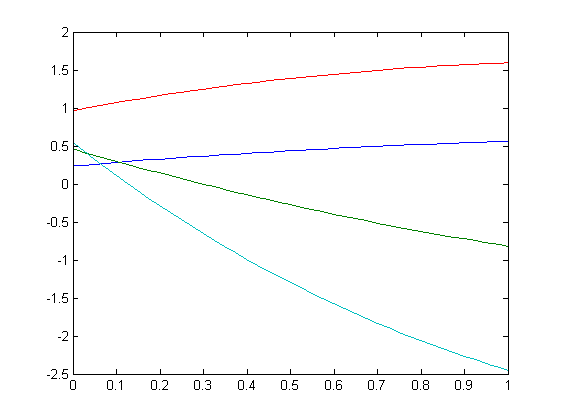
\includegraphics[scale=0.5]{example_plot.png}
\caption{Graph presenting data from Table \ref{sampleData} \label{samplePlot}, Time$\times X$.}
\end{figure}
	\subsection{Creating movies}
    Matlab provides a tool set for creating animated movies. The concept is that a movie is a set of images called frames. Each frame, which is a 3-dimensional image for coloured images, is stored in a 2-dimensional array which contains 3-dimensional frames. Eventually, the result is a 4-dimensional array of size $ F\times X\times Y\times 3 $, with F being the number of frames, $ X\times Y $ the size of each frame and number 3 the vector size of colour values in RGB colour model. 
    
To create a movie, Matlab needs to record images from a figure type window. Thus, for every frame stored, an image must be shown in the same figure window. The function that creates and shows an image out of a 2-3D matrix is called imshow(M), M is the argument that represents a 2-dimensional or 3-dimensional matrix (2D for grey-coloured images, 3D for coloured). Then the function \texttt{getFrame(Figure,window-size)} is called, in order to grab the frame. All frames must be stored in a matrix that was initialised by the function \texttt{moviein(numberOfFrames,Figure,windowSize)}. 
    
Every structure of type `Figure' has an identifier. Thus, keeping the same identifier for the figure that hosts the image from \texttt{imshow()} avoids the creation of many windows. The result is one figure-window that hosts a different image while time passes, resulting in an animated movie show. A structure of type `Figure' is constructed by calling the function \texttt{figure(id)} with \texttt{id} being a natural number. The general function playMovie that was developed can be viewed in Appendix section \ref{playmovie}.

    \subsubsection{Creating the images}
    
Alan Turing states that morphogens are chemical compounds that give certain characteristics to the cells according to their type and concentration \cite{turing_chemical_1990}.
A way to identify and differentiate cells in a computer simulation is to give them different colours according to their morphogen concentrations. Many ideas and combinations were used on how to match morphogen concentrations to different colours. 
    
The first problem in matching morphogen concentrations to colour values is to normalise the concentrations, which are arbitrary real values greater than 0, to real values in the range $ [0,1] $. The Algorithm \ref{colorsmap} describes the colour-mapping procedure.

\begin{algorithm}                      
\caption{Colour mapping}          
\label{colorsmap}                          
\begin{algorithmic}                    
    \STATE{let MORPHOGENS be a 2D array of positive real values}
    \STATE{let MIN be the minimum value in MORPHOGENS}
    \STATE{let MAX be the maximum value in MORPHOGENS}
    \STATE{let an array COLOURS be the same dimensions as the MORPHOGENS array's}    
    \FOR{each VALUE in MORPHOGENS}
        \STATE{NEWVALUE=(VALUE-MIN)/(MAX-MIN)}
        \STATE{add the NEWVALUE to COLOURS}
    \ENDFOR
\end{algorithmic}
\end{algorithm}    

After converting the concentration values in colour values and storing them in a 3-dimensional array, the \texttt{imshow()} method will output a coloured image of a representation of the cells at a certain point in time. This is called a snapshot of the state of the physical system under study.
	\subsection{Producing sound}

    Since models of morphogenesis present an oscillatory behaviour, the wave patterns that are obtained can be mapped into sound waves. A model with continuous/persisting oscillations is the Gizburg-Landau model which involves partial differential equations. The template for computing the mathematical model is given by Aly-Khan Kassam \cite{kassam_solving_2003}.
    
    The morphogen values can be imported directly to the Matlab function \texttt{soundsc(values, sample rate, bit depth)}, that normalises and scales them automatically to sound values. Decreasing the sample rate makes the sound heavier/slower, while higher sample rates make the sound accute. Matlab documentation states that the \texttt{soundsc} function accepts sample rates of the range $[80,10^6]$ \cite{MATLAB_2010} but it is bound on what the sound card on the machine can support.

    The \texttt{soundsc} is available on both Windows and UNIX architectures. The implementation was done on a Linux-based operating system (Fedora 17) and the method used the ALSA drivers to generate sound. 


	\section{Java}
    One of the goals of the project was to identify ideas based on morphogenesis that can be applied to computer science or other engineering problems. Java was chosen as the tool to deliver such solutions, since it can work on many machines and on various operating systems. In addition, Java is more suitable for Object Oriented Programming (OOP) than Matlab. Matlab supports OOP as well, but two main reasons led to the decision of chosing Java over Matlab.
    \begin{enumerate}
    \item The fact that type handling in Java is explicit, helps in a better structural software design, with the use of various patterns as described by the Gang of Four \cite{gamma_design_1998} and GRASP\footnote{GRASP is an acronym for General Responsibility Assignment Software Patterns \cite{larman_applying_2004}} principles \cite{larman_applying_2004} 
resulting to a more understandable, easy to maintain source code.
    \item Matlab is proprietary software and since no explicit Matlab tools are needed, Java is the best way to deliver, develop and expand free, easy-to-implement and use software framework.
    \end{enumerate}

    The solution is broken into two main concepts: Building an ODE solver and a simulation of process management system. The idea is described in paragraph \ref{disch}, Diffusion inspired scheduler.    

	\subsection{Implementing Euler's method}
    
A method for integrating ordinary differential equations is the Euler's method. Euler's method is a first order method \cite{koch_implicit_2000}. Two ways to implement the Euler's method are suggested. The approach that was proposed originally is the explicit method where the time-step is fixed. A more advanced solution is the implementation of implicit methods which change dynamically the time steps to reduce integration errors during steps. 

Euler's method is used for the purpose of the diffusion scheduling. Since there is a limit on the time slice,
the explicit method is used to avoid the disadvantage of increasing the total complexity of the algorithm.
That means that the error per step is proportional to the square of the step size. To approximate the reaction-diffusion model of L-systems, a step of 0.1 time units is considered as suggested and implemented from Christopher G. Jennings, PhD in his work on Turing's Reaction-Diffusion Model of Morphogenesis \cite{website:jennings}. 
    
The method takes the initial values for every variable in a vector $ x_0 $ of size N.
    $$ \dot{x}_0 = \begin{pmatrix}
x_1 \\ 
\vdots \\
x_n \\
\end{pmatrix}
$$ 
    Then, for each time step, starting from $ n = 0 $ it calculates the next state in the next time step.
    $$ \dot{x}_{n+1} = \dot{x}_n + h*f(t_n, \dot{x}_n) $$
    
Where:
\begin{itemize}
\item h is the step size and it should be less than 1.
\item n is the index to the current step.
\end{itemize}    

The algorithm that describes the implementation of the Euler's method is shown in Figure \ref{euleralgo}. The algorithm depends on the function and its number of variables. For that reason, the Template pattern was used to protect the implementation of the Euler's method from function variations. As shown in Appendix \ref{App:AppendixB}, the abstract class AbstractFunction provides a default implementation of an equation. In order to add a new equation, a new class has to be implemented that extends the AbstractFunction. Thus, by the means of inheritance, the variations of different equations are hidden from the ODE solver resulting in a coherent code that does not need to change every time a new equation is added. 

Likewise, ODE solvers can be added, as defined by the ODE interface, without the need of changing the functions since the ODE interface and the AbstractODE is bound to the AbstractFunction. In other words, the principle of GRASP for protecting variations was widely taken into account to construct a well coherent framework.

\begin{algorithm}                      
\caption{Euler's method}          
\label{euleralgo}                          
\begin{algorithmic}
    \STATE{results[0]=initial conditions}                    
    \FOR{i in 1 to number of total steps}
			\STATE{results[i] = results[i-1] + timestep*function()}
    \ENDFOR
    \STATE{return results}
\end{algorithmic}
\end{algorithm}

    \subsection{Process management}

A process is a portion of code that needs to be executed by a processor to accomplish a task. This execution needs time to be completed, proportional to the cycles per second that the processor runs.

The process management is a responsibility of the operating system. Each operating system can have one or more scheduling algorithms to manage the execution of a queue of processes. Modern operating systems, support preemptive multitasking \cite{tanenbaum_modern_2007}. This means, that a process can be paused without its permission and another process can take its place. The scheduling algorithms become more sophisticated in order to handle pseudo-parallelism. The general goal is to keep each process as less idle as possible.

This project explores the behaviour of executing a fixed amount of processes by using a diffusion-inspired scheduler as described in paragraph \ref{disch} 
against other process schedulers. The study is just an introduction to the idea of using the concept of reaction-diffusion to help the algorithm decide on how much time each process must be given each turn.
Each process has the properties described in Figure \ref{processfigure}. 

The processes are arranged in a queue. No new processes are added in the queue and a process is removed from the queue when it exits with a finished or a crash message.
\begin{figure}
\centering
\includegraphics[scale=0.8]{process_figure.png}
\caption{Scheme of a process as handled by the implementation of the process management framework.}
\label{processfigure}
\end{figure}


	\subsection{The scheduling problem}	
\label{schedulers}
The responsibility of a scheduler is to find a way of executing all the processes that seek execution time with maximum efficiency. The term efficient is ambiguous but justifiably so. The goal of a scheduler differs from situation to situation and from system to system. Despite the fact that in a distributed system, prioritising might be less important than executing client requests without the concern of which client should get the response first. There are also some general specifications that a scheduler shall achieve.
Some general goals include:
\begin{itemize}
\item To finish as early as possible.
\item To execute system processes with higher priority.
\item To avoid starvation.
\item To detect deadlocks.
\end{itemize}
Finishing fast is not as crucial as it may seem. It is clear, that the fastest solution in terms of time is to execute the processes serially (assuming all finish at some point). However, the most important concept in a real-world situation is to present pseudo-parallelism, that is to make the processes look that they are being executed in parallel. 
Avoiding starvation is another specification a scheduler has to offer. Assuming that the body of the code under processing does not contain any deadlock situations, then all processes must be executed and finished at some point in time. Thus, each process should take some time in every short amount of cycles. The phenomenon on which a process is not given processing time at all is called starvation. 

Deadlocks are not considered in this project but they should be referenced to avoid conflicts with starvation. A deadlock can occur when two or more processes wait for each other to continue their processing. If this happens, the scheduler will be running those processes forever. Detection of deadlocks is important but is not always the responsibility of the scheduler. Usually, the program that detects deadlocks is called `watchdog' \cite{tanenbaum_modern_2007}. However, it is crucial for a scheduler to work smoothly if deadlocks are detected to avoid wasting time with frozen processes.

The rest of the Chapter describes different scheduler algorithms used to assess the performance of the diffusion-inspired scheduler. These are the random sceduler, the Round-Robin and the priority scheduler. The algorithm of the diffusion-inspired scheduler is also given.
	
\subsubsection{Random scheduler}
The random scheduler picks randomly a process from the queue and executes it for a fixed amount of time units. The pseudo-code is in Algorithm \ref{RandSch} below.


\begin{algorithm}                      
\caption{Random scheduler}          
\label{RandSch}                           % and a label for \ref{} commands later in the document
\begin{algorithmic}                    
    \WHILE {Process queue is not empty}
        \STATE{choose a process at random}
        \STATE{ask the process to run up to a pre-defined number of time units}
        \STATE{get acknowledgment message from process}
        \STATE{get time used by the process}
        \STATE{increase for each other process their idle time}
        \STATE{increase execution time for the process chosen}
        \IF {the process finished}
            \STATE{add execution time, idle time and total time to the scheduler statistics}
            \STATE{remove process from queue}
        
        \ENDIF
    
    \ENDWHILE
    \STATE{display statistics}    
\end{algorithmic}
\end{algorithm}


	\subsubsection{Round Robin scheduler}
The Round Robin scheduler picks serially each process in the queue and executes it for a fixed amount of time units. It guarantees that eventually all processes will be executed and exit. The pseudo-code is shown in the Algorithm \ref{RRSch}.

\begin{algorithm}[H]                      
\caption{Round Robin scheduler}          
\label{RRSch}                           % and a label for \ref{} commands later in the document
\begin{algorithmic}                    
    \WHILE{Process queue is not empty}
        \STATE{choose next process in queue}
        \STATE{ask the process to run up to a pre-defined number of time units}
        \STATE{get acknowledgment message from process}
        \STATE{get time used by the process}
        \STATE{increase for each other process their idle time}
        \STATE{increase execution time for the process chosen}
        \IF{the process finished}
            \STATE{add execution time, idle time and total time to the scheduler statistics}
            \STATE{remove process from queue}
        
        \ENDIF
        \IF{last process in queue}
            \STATE{set pointer back to the start}
        \ENDIF
    
    \ENDWHILE
    \STATE{display statistics}    
\end{algorithmic}
\end{algorithm}
 
	\subsubsection{Priority scheduling}
The priority scheduler is based on the fact that some processes are more important than others. The implementation assigns a random integer 0-39 to each process in the waiting queue. This is the priority of the process; the smaller the number the higher the priority. The scheduler executes serially the processes with the minimum priority number until they are all finished and then moves on to the next minimum priority number until the queue is empty. The pseudo-code is shown in Algorithm \ref{PRSch}.

\begin{algorithm}                      
\caption{Priority scheduler}          
\label{PRSch}                           % and a label for \ref{} commands later in the document
\begin{algorithmic}      
    \STATE{set a priority value from 0-39 for each process}              
    \STATE{set minimum value to 0}    
    \WHILE{Process queue is not empty}
        \IF{a process with priority equal to the minimum value does not exist in the queue} 
        \STATE{find the minimum priority value of a process existing in the process queue}
        \ENDIF        
        \STATE{find the next process with priority value equal to the minimum value}
                
        \STATE{ask the process to run up to a pre-defined number of time units}
        \STATE{get acknowledgment message from process}
        \STATE{get time used by the process}
        \STATE{increase for each other process their idle time}
        \STATE{increase execution time for the process chosen}
        \IF{the process finished}
        \STATE{add execution time, idle time and total time to the scheduler statistics}
        \STATE{remove process from queue}
        
        \ENDIF
    
    \ENDWHILE
    
    \STATE{display statistics}    
\end{algorithmic}
\end{algorithm}
	\subsubsection{Diffusion-inspired scheduler}
\label{disch}
The implementation of the diffusion-inspired scheduler exploits the idea of the Round Robin in an alternative implementation of a weighted Round Robin scheduler. That is, instead of having a fixed amount of time units that a process takes to be executed, the time varies according to Diffusion dynamics. The advantage is that because of diffusion all processes are guaranteed to take some time but not necessarily on every execution round. 

The processes are initially given a certain random time unit value that is in reality the amount of time that it will be given for execution. That amount of time represents the concentration of a morphogen in a physical system of cells, and thus, processes represent cells. The processes are executed for the amount of time units given. After the execution round ends, the reaction-diffusion dynamics are calculated and the system of equations is integrated giving as a result new time units for each process.

An exceptional scenario can be encountered where processes starve. This can happen when all the processes that have a positive time unit are executed and finish, leaving in the queue processes that have 0 time units and are thus unable to diffuse. This is solved by following a simple rule: if a process is called to be executed for 0 time cycles, then it is always executed for one.

A more sophisticated way to avoid starvation is to assign two fixed pseudo-processes to certain places in the queue that have a fixed amount of time units that never change, and thus feeding the rest of the processes avoiding starvation. These scenarios and solutions were not studied. Nevertheless, the fact that starvation did not happen during the experiments points that further investigation is needed. The implemented framework is freely available for expansions and testing various ideas. 

The algorithm of the Diffusion scheduler is provided below (Algorithm \ref{DSch} ).

\begin{algorithm}                      
\caption{Diffusion-inspired scheduler}          
\label{DSch}                           % and a label for \ref{} commands later in the document
\begin{algorithmic}
    \STATE{set randomly time units to a process in a range close to the other ranges

    (alternatively, set equal time units to a process equal to the pre-defined value)}                    
    \WHILE{Process queue is not empty}
        \STATE{choose next process in queue}
        \STATE{ask the process to run up to its given number of time units}
        \STATE{get acknowledgment message from process}
        \STATE{get time used by the process}
        \IF {process used all the time}
        \STATE{set the reaction variable of that process to 0}
        \ENDIF
        \IF {process was last in queue}
        \STATE{set Euler time step to 0.01 as an imaginary time step}
        \STATE{calculate reaction-diffusion differential equations
                by applying Euler's method and assign to each process
                a new amount of time units}

        \ENDIF
        \STATE{increase for each other process their idle time}
        \STATE{increase execution time for the process chosen}
        \IF{the process finished}
        \STATE{add execution time, idle time and total time to the scheduler statistics}
        \STATE{remove process from queue}
        \ENDIF
        \IF{last process in queue}
        \STATE{ set pointer back to the start}
        \ENDIF
    
    \ENDWHILE
    \STATE{display statistics}    
\end{algorithmic}
\end{algorithm}

Development description of the process management framework is given in Chapter \ref{softD}.
